% !TEX root = thesis.tex
\section{Analysis method}
\label{sec:methods}

\subsection{Jet Finders}


The analysis is performed by analysing jet constituents. In each collision event, the jets are reconstructed using FastJet~\cite{fastjet} with the anti-$\kt{}$ algorithm~\cite{antikt}. Jets for R=0.4 are selected in $\left| \eta \right| < 0.25 $ to satisfy the fiducial acceptance of the EMCal.In jet reconstruction both charged tracks with $\pt{}>0.15\,\GeVc$ and neutral cluster with $\pt{}>0.30\,\GeVc$ are considered. In the analysis, results are presented in terms of the jet transverse momentum $\pt{jet}$.

\subsection{$j_T$ }


The jet fragmentation transverse momentum, $\jt{}$, is defined as the component of the constituent particle momentum, $\vec{p}_{\mathrm{a}}$, transverse to the jet momentum, $\vec{p}_{\mathrm{jet}}$. The resulting $\vjt{}$ is illustrated in~\fig{fig:jtdefinition}. The length of the $\vjt{}$ vector is
  \begin{equation}
    \jt{} = \frac{|\vec{p}_{\mathrm{jet}} \times \vec{p}_{\mathrm{track}}|}{|\vec{p}_{\mathrm{jet}}|} \,.
  \label{eq:jtdefinition}
  \end{equation}

It is commonly interpreted as a transverse kick with respect to the initial hard parton momentum that is given to a fragmenting particle during the fragmentation process, which is a measure of the momentum spread of the jet fragments~\cite{}. 

   \begin{figure}
    \begin{center}
      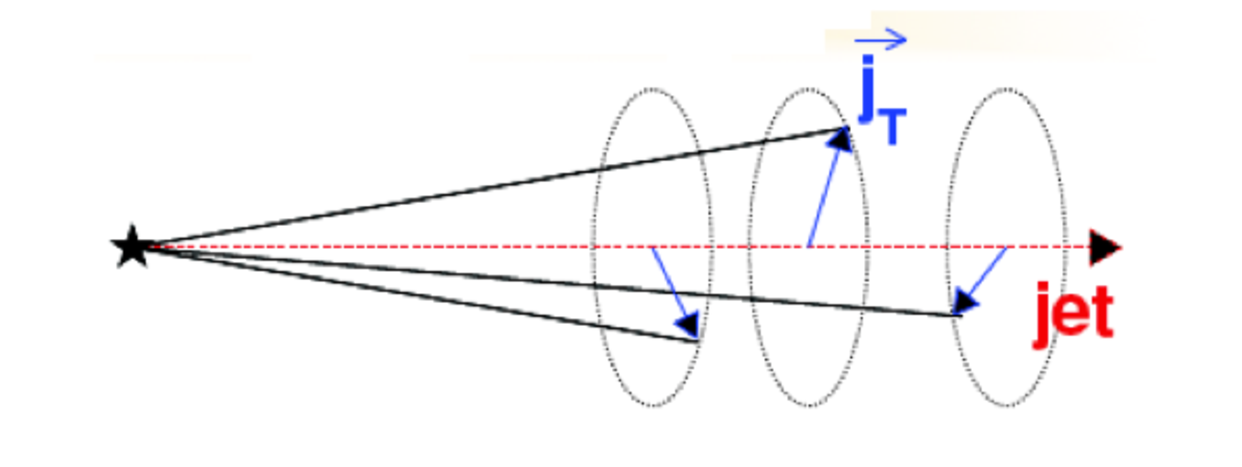
\includegraphics[width = 0.60\textwidth]{figures/jt_def}
    \end{center}
    \caption{Illustration of $\vjt{}$. The jet fragmentation transverse momentum, $\vjt{}$, is defined as the transverse momentum component of the track momentum, $\vec{p}_{\mathrm{track}}$, with respect to the jet momentum, $\vec{p}_{\mathrm{jet}}$.}
    \label{fig:jtdefinition}
  \end{figure}

The reconstructed jet axis is used for $\jt{}$ reference. Any charged track within a fixed cone with radius $R$ is taken as a jet constituent, as opposed to using the constituent list provided by the jet algorithm. Anti-$\kt{}$ produces jets that are very circular in shape. Thus this doesn't change the constituent list considerably. Neutral tracks are used only in jet reconstruction.
 
 \subsection{Unfolding}
{\color{red} Extend unfolding}
 
The resulting $\jt{}$ distributions are corrected for the detector inefficiency using the unfolding method. The response matrix for the unfolding is obtained from a \textsc{Pythia}~\cite{introPythia81} simulation.
 

 
 \subsection{Background}

 
The underlying event is estimated by looking at an imaginary jet cone perpendicular to the observed jet axis ($\frac{\pi}{2}$ Rotation in $\phi$). $\jt{}$ is calculated for any tracks found within this cone. The vector sum of the individual track momentum and the imaginary jet axis is used as reference for $\jt{}$. The background obtained in this manner is subtracted from the unfolded inclusive $\jt{}$ distribution, which gives the resulting signal distribution. To make sure there is no jet contribution in the background, any events with jets inside the perpendicular cone are not used for background estimation.

{\color{red} Extend Background, Perp. cone vs. Random}


 \subsection{Fitting}


The resulting signal distribution are fitted with a 2 component function shown in Eq.~\ref{eq:fit}. Gaussian distribution is used for low $\jt{}$ and an inverse gamma function is used for high $\jt{}$. The gaussian is taken to have the center at $\jt{} = 0$. In total this gives 5 parameters.

\begin{equation}
\frac{1}{N_{\mathrm{jets}}}\frac{\mathrm{d}N}{\jt{} \mathrm{d}\jt{}} = \frac{B_2}{B_1\sqrt{2\pi}}e^{-\frac{\jt{}^2}{2B_1^2}}+\frac{B_3B_5^{B_4}}{\Gamma\left(B_4\right)}\frac{e^{-\frac{B_5}{\jt{}}}}{\jt{}^{B_4+1}}
\label{eq:fit}
\end{equation}

To achieve stable results the fitting is performed in two steps. First each component is fitted separately. Gaussian component is fitted to the low end in $\jt{}$. Inverse gamma component is fitted to $\jt{}$ above $\unit[1]{\gevc}$. After getting the results from the individual fits they are combined into a single function with initial values from the individual results and an additional fit is performed. Fitting only the gaussian component to the entire distribution produces approximately the same result as the gaussian component in the two-component model.

After getting the fit function $\sqrt{\left<\jt{}^2\right>}$ (RMS) and yield values are  extracted separately from each component. The narrow component RMS is

$$\sqrt{\left<\jt{}^2\right>}=\sqrt{2}B_1,$$

and the wide component RMS value is calculated as 

$$\sqrt{\left<\jt{}^2\right>}=\frac{B_5}{\sqrt{\left(B_4-2\right)\left(B_4-3\right)}},$$

where it is required that $B_4 > 3$.

\section{Systematic uncertainties}
{\color{red} Extend Systematics}

\label{sec:systematicerrors}
The systematic uncertainties in this analysis come from the background estimation, the unfolding procedure and the cuts used to select the tracks. Tracking uncertainties are estimated from variations of the track selection cuts defined in Sec.~\ref{sec:experimentaldetails}. The resulting variations in RMS are shown in Table \ref{tab:systematics}. The uncertainties from unfolding and background subtraction are of the same magnitude. 

The systematics in background estimation were studied using an alternative method to extract the background, mainly the random background method. The resulting uncertainty is below 5\% for the wide component RMS and below 9\% for the narrow component RMS. 

The systematic uncertainty that arises from the unfolding procedure is estimated by performing the unfolding with two separate methods. Data corrected by the iterative unfolding method are used as the results and the SVD unfolding method is employed to estimate the uncertainty. In a \textsc{Pythia} closure test the true distribution was in general found to be between the unfolded distributions from the iterative and SVD method. The difference between the methods when unfolding data should give a reasonable estimate of the unfolding uncertainty. The resulting uncertainty is below 8\% for both wide and narrow component RMS.

The different source of the systematic uncertainty are considered as uncorrelated and the values of each source are summed in quadrature. The resulting uncertainty is 9 \% for the wide component RMS and 12 \% for the narrow component RMS. 

\begin{table}[htb]
\centering
\caption{Summary of systematic errors}
\label{tab:systematics}
\begin{tabular}{ l | c | r }
  Systematic & Wide RMS & Narrow RMS \\
    \hline			
  Background & 5 \% & 9 \% \\
  Unfolding & 8 \% & 8 \% \\
  Tracking & ? \% & ? \% \\
  Total & 9 \% & 12\% \\
  \hline
  \end{tabular}
  \end{table}

There is no tracking and no unfolding uncertainty in the Monte Carlo simulations. 